% Supplementary methods, complete operating points, and control comparisons.
% Generated table blocks are populated from the numerical results.
\appendix
\section{Experimental Inventory}
\label{app:inventory}
Table~\ref{tab:cohorts} separates independent inputs from their reuse across
estimators and decoders. Diagnostic blocks contain multiple strategies, each
charged its complete transmitted-signal budget. The precision grid uses fresh
acquisitions even at conditions shared with the cross-circuit study.

% BEGIN GENERATED COHORT_TABLE
\begin{table}[!htbp]
\centering
\small\setlength{\tabcolsep}{4pt}
\caption{Experimental map. Frame counts denote distinct inputs before reuse across priors, codes, or decoders. A diagnostic replicate block evaluates several fully budgeted acquisition strategies and produces no key. The 450 symmetric reference-calibration frames are additional. Detailed grids and reuse rules are given in the methods and supplement. Target profiles additionally reuse 2500 held-out-validation fitting records, without new acquisitions.}
\label{tab:cohorts}
\begin{tabular}{@{}lllr@{}}
\toprule
Cohort & Resource & Outcome & Inputs \\
\midrule
Circuit & $n=1000,S=200$ & FER and yield & 68,000 \\
Pooling/rate development & Varied $n,S$ & Frozen rules & 25,800 \\
Pooling confirmation & $n=1000$, varied $S$ & Fixed-code yield & 37,500 \\
Code transfer & $n=1000,4000,16000$ & Prior/policy yield & 22,500 \\
Sample allocation & $n+S=2000$ & Total yield & 12,500 \\
Physical controls & $n=1000,S=200$ & Conditional priors & 25,000 \\
Diagnostic reference/stress & Varied $T$ & Residual and coverage & 45,000 \\
Basis/range validation & Varied $T$; held-out setting & Residual and prediction & 31,000 \\
Full-data/circuit validation & $T=8000$ per strategy & Residual and coverage & 6,500 \\
Budget/interception validation & Varied $T,r$ & Precision contrasts & 40,500 \\
\bottomrule
\end{tabular}
\end{table}
% END GENERATED COHORT_TABLE
\FloatBarrier

\subsection{Uncertainty and computational checks}
Absolute FERs include failure counts and Wilson 95\% intervals~\cite{wilson1927}.
Exact two-sided McNemar tests use paired rescued/harmed frames. Holm correction covers
12 circuit cells separately for each decoder, and 75 confirmation cells separately for
each comparator. Paired bootstrap yield intervals (10,000 resamples) condition on each frozen matrix and
calibration choice; they do not include retraining uncertainty.

For transfer and physical/sample controls, the five matrix libraries are the units for
generalization. We report $t_4$ intervals on their paired mean yield differences, with
within-matrix frame uncertainty supplied separately. These exploratory intervals are
not adjusted across conditions. Zero observed discordance can collapse a bootstrap
interval at zero; it does not exclude rare harms. Grid means weight design cells equally
and are not population averages for a deployment.

Protocol-derived inventories count reused input frames only once. Independent
density-state calculations, decoder references, and retained-record checks verify
the implementation. Reproduction checks match all 1504 retained circuit-study arrays;
decoder audits cover every confirmation and transfer/control holdout and selected
development records. Diagnostic checks cover retained counts and budgets, density-state
responses, and independent reference fits. Fresh full runs match all 6670 retained range-validation arrays, all 1090
full-observation arrays, and all 3078 precision-grid arrays exactly. The full-observation study checks cross-circuit response
laws, analytic inverses, likelihood optima, and profile endpoints against
independent numerical references. The supplement specifies the
random-number generators, seeds, and exact verification scopes; cohort totals appear
in Appendix~\ref{app:rule}. Information benchmarks and yield decompositions are
descriptive calculations on the fixed evaluation records, not inputs used to tune
the selected rules. Entropies are checked both from joint probabilities and from
binary-transition formulas; the yield identity is checked for every paired frame.


\FloatBarrier
\section{Circuit Operating Points and Robustness}
\label{app:circuit}
\label{app:ablation}
The circuit study contains 6000 calibration frames, 24,000 main holdout frames,
6000 matrix-replication frames, 12,000 fixed-curve frames, and 20,000 channel
calibration/holdout frames. Reusing those frames across priors, decoders, and fixed-code
analyses does not create additional independent inputs. The matched comparison appears in Table~\ref{tab:matched};
Table~\ref{tab:operating} reports every calibrated operating point. The observed FER is below 1\% in all
12 main cells for both BP policies, although not every upper confidence bound is
below that threshold. The efficiencies describe this conservative finite-length
family and do not establish competitiveness with optimized QKD codes.

\subsection{Codes, calibration and circuit controls}
The circuit study uses a nested column-weight-three, progressive-edge-growth-style
family~\cite{hu2005}. Starting at 150 checks on 1000 variables, splitting a check into
two disjoint parts preserves nesting and gives $m=150,175,\ldots,900$. All 93 stored
matrices have full row rank. Layered sum-product belief propagation (BP) runs for at most 300 sweeps.
A stronger comparator adds full order-one ordered-statistics decoding (OSD)
\cite{fossorier1995} on nonconvergence or failed public verification, with the same search
budget for both priors. Simulator correctness never triggers the retry.

For each encoding and $Q\in\{0.02,0.06,0.10\}$, 500 calibration frames select the
smallest tested row count whose Wilson 95\% upper FER bound is at most 1\%, provided
all higher tested counts also pass. Pooled and shrinkage policies select separately.
Their choices are frozen before 2000 holdout frames per cell, giving 24,000 main
holdout frames. Fixed-code comparisons use the same shrinkage-selected matrix for
both priors; operating-policy comparisons allow their selected row counts to differ.
Two further matrix seeds, fixed-code curves, and link-noise controls complete the
68,000-frame circuit study.
A post hoc fixed-code sensitivity analysis replaces gate noise with isotropic link
noise at constant total QBER. It uses the gate-calibrated matrices to avoid the
near-zero failure floor of adaptive channel policies; channel outcomes do not
determine the selected matrices.


\begin{equation}
 f_{\mathrm{syn}}=\frac{m}{nh_2(Q)},\qquad
 f_{\mathrm{EC}}=\frac{m+64}{nh_2(Q)}.
 \label{eq:efficiency}
\end{equation}
Here $h_2(x)=-x\log_2x-(1-x)\log_2(1-x)$ is binary entropy, with $0\log_2 0=0$.
These disclosure efficiencies use the measured retained-block QBER in the
circuit study. Every transmitted syndrome row is charged, including dependent
rows. Authentication and privacy amplification are outside $Y$.
\subsection{Matched-code and operating comparisons}
\begin{table}[htbp]
\centering
\small\setlength{\tabcolsep}{3.2pt}
\caption{Matched-code comparisons at 10\% target QBER. Both priors use the shrinkage-selected matrix and the same 2000 frames. P/S denote pooled/shrinkage priors. Counts accompany absolute FER; R/H are rescued/harmed pairs. Ratios include paired bootstrap 95\% intervals when at least five pooled failures support estimation; a dash indicates an undefined or too-sparse ratio interval. Holm correction covers the 12 main cells separately for BP and BP+OSD.}
\label{tab:matched}
\begin{tabular}{@{}llcllccc@{}}
\toprule
Encoding & Decoder & $m$ & FER P (\%) & FER S (\%) & R/H & Ratio [95\% CI] & $p_{\rm Holm}$ \\
\midrule
Standard & BP & 625 & 112: 5.60 [4.67, 6.70] & 11: 0.55 [0.31, 0.98] & 102/1 & 0.098 [0.05, 0.16] & 2.5e-28 \\
Standard & BP+OSD & 625 & 88: 4.40 [3.59, 5.39] & 8: 0.40 [0.20, 0.79] & 81/1 & 0.091 [0.03, 0.16] & 4.1e-22 \\
A & BP & 650 & 33: 1.65 [1.18, 2.31] & 19: 0.95 [0.61, 1.48] & 16/2 & 0.576 [0.38, 0.78] & 0.014 \\
A & BP+OSD & 650 & 28: 1.40 [0.97, 2.02] & 13: 0.65 [0.38, 1.11] & 17/2 & 0.464 [0.26, 0.69] & 0.008 \\
B & BP & 675 & 3: 0.15 [0.05, 0.44] & 4: 0.20 [0.08, 0.51] & 0/1 & 1.333 [--] & 1 \\
B & BP+OSD & 675 & 1: 0.05 [0.01, 0.28] & 2: 0.10 [0.03, 0.36] & 0/1 & 2.000 [--] & 1 \\
B+ & BP & 700 & 0: 0.00 [0.00, 0.19] & 1: 0.05 [0.01, 0.28] & 0/1 & -- [--] & 1 \\
B+ & BP+OSD & 700 & 0: 0.00 [0.00, 0.19] & 1: 0.05 [0.01, 0.28] & 0/1 & -- [--] & 1 \\
\bottomrule
\end{tabular}
\end{table}
Operating-policy gains answer a different question because the selected syndrome lengths
can differ. In Scheme~A at 10\% QBER, pooled and shrinkage BP select 700 and 650
rows, respectively; their yield difference is +3.94 percentage points (pp), with paired
95\% interval [+3.83, +4.04]. The smaller syndrome comes with 19 failures versus
zero: shrinkage FER is 0.95\%, with Wilson interval [0.61\%,1.48\%]. Although
the point estimate is below 1\%, its upper bound exceeds the calibration criterion,
so the holdout does not establish the targeted reliability. The gain is largely a
disclosure effect conditional on that calibration. At 2\% QBER the same procedure loses 4.09 pp, and balanced B+ loses
2.00 pp at 10\%. Table~\ref{tab:operating} reports every operating cell, including
absolute FER and disclosure efficiency. These losses motivate a rule that can return
to pooling when the sample is uninformative.

\begin{table}[htbp]
\centering
\small\setlength{\tabcolsep}{3.2pt}
\caption{Main BP operating policies. Each cell has 2000 independent holdout frames. FER entries give failure counts, percentages, and Wilson 95\% intervals. P denotes pooled priors and S centred shrinkage. $m$ and $f_{\mathrm{EC}}$ are shown as P/S pairs. Yield differences and paired 95\% intervals are in percentage points. Target QBER labels denote generator expectations.}
\label{tab:operating}
\begin{tabular}{@{}lcccllc@{}}
\toprule
Encoding & $Q$ (\%) & $m$ P/S & $f_{\mathrm{EC}}$ P/S & FER P (\%) & FER S (\%) & $\Delta Y$ (pp) \\
\midrule
Standard & 2 & 400/400 & 3.29/3.29 & 0: 0.00 [0.00, 0.19] & 0: 0.00 [0.00, 0.19] & +0.00 [+0.00, +0.00] \\
Standard & 6 & 550/525 & 1.88/1.80 & 0: 0.00 [0.00, 0.19] & 1: 0.05 [0.01, 0.28] & +2.07 [+2.03, +2.08] \\
Standard & 10 & 700/625 & 1.63/1.47 & 1: 0.05 [0.01, 0.28] & 11: 0.55 [0.31, 0.98] & +6.12 [+6.03, +6.19] \\
A & 2 & 300/350 & 2.57/2.92 & 4: 0.20 [0.08, 0.51] & 1: 0.05 [0.01, 0.28] & -4.09 [-4.16, -3.98] \\
A & 6 & 550/525 & 1.87/1.80 & 3: 0.15 [0.05, 0.44] & 5: 0.25 [0.11, 0.58] & +2.05 [+1.96, +2.13] \\
A & 10 & 700/650 & 1.63/1.52 & 0: 0.00 [0.00, 0.19] & 19: 0.95 [0.61, 1.48] & +3.94 [+3.83, +4.04] \\
B & 2 & 300/300 & 2.56/2.56 & 9: 0.45 [0.24, 0.85] & 7: 0.35 [0.17, 0.72] & +0.05 [-0.05, +0.16] \\
B & 6 & 525/525 & 1.80/1.80 & 8: 0.40 [0.20, 0.79] & 9: 0.45 [0.24, 0.85] & -0.02 [-0.05, +0.00] \\
B & 10 & 675/675 & 1.58/1.58 & 3: 0.15 [0.05, 0.44] & 4: 0.20 [0.08, 0.51] & -0.01 [-0.03, +0.00] \\
B+ & 2 & 375/375 & 3.12/3.12 & 0: 0.00 [0.00, 0.19] & 0: 0.00 [0.00, 0.19] & +0.00 [+0.00, +0.00] \\
B+ & 6 & 525/525 & 1.81/1.81 & 7: 0.35 [0.17, 0.72] & 7: 0.35 [0.17, 0.72] & +0.00 [+0.00, +0.00] \\
B+ & 10 & 675/700 & 1.58/1.63 & 9: 0.45 [0.24, 0.85] & 1: 0.05 [0.01, 0.28] & -2.00 [-2.06, -1.92] \\
\bottomrule
\end{tabular}
\end{table}


Figure~\ref{fig:exposure} compares path-model predictions with measured basis probabilities.
Figure~\ref{fig:curves} evaluates fixed codes across QBER, avoiding changes in code profile
within a curve. Their purpose is to expose the mechanism and operating regime rather than
maximize a single failure ratio.

\begin{figure}[htbp]
\centering
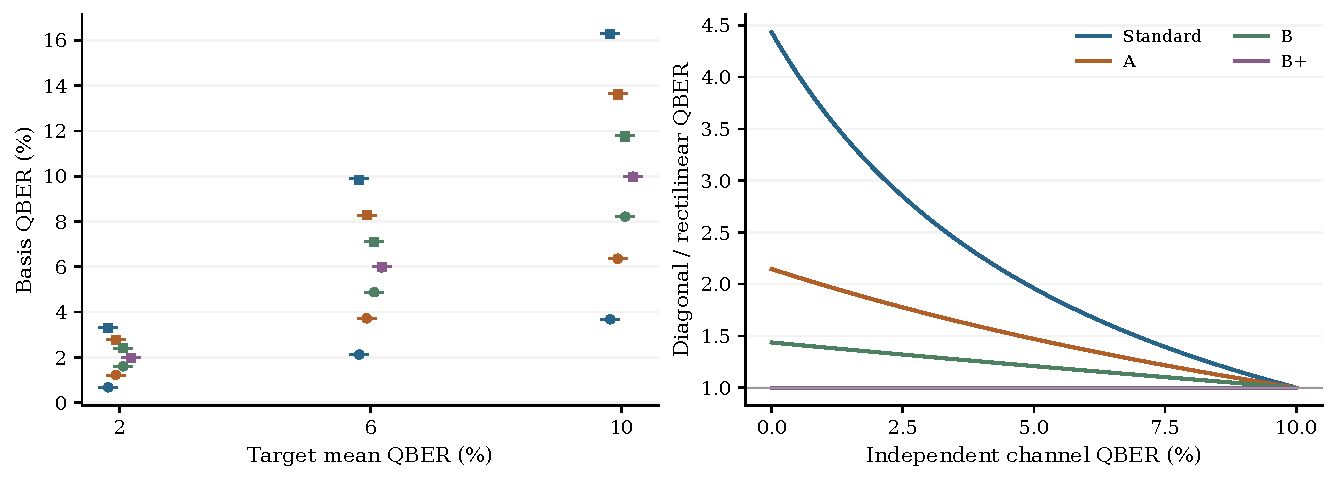
\includegraphics[width=0.94\linewidth]{images/gate_exposure.pdf}
\caption{Left: measured basis QBERs across the main holdout frames; circles indicate rectilinear and squares diagonal. Colors follow Standard, A, B, and B+ as in the legend at right. Short horizontal marks give exact gate-model predictions. Wilson 95\% error bars are smaller than most markers because each point pools approximately 1.2 million bits. Right: predicted attenuation of the basis ratio when channel noise replaces gate noise at fixed 10\% total QBER.}
\Description{Basis error probabilities agree with gate-count predictions; independent channel noise drives each diagonal-to-rectilinear ratio to one.}
\label{fig:exposure}
\end{figure}

\begin{figure}[htbp]
\centering
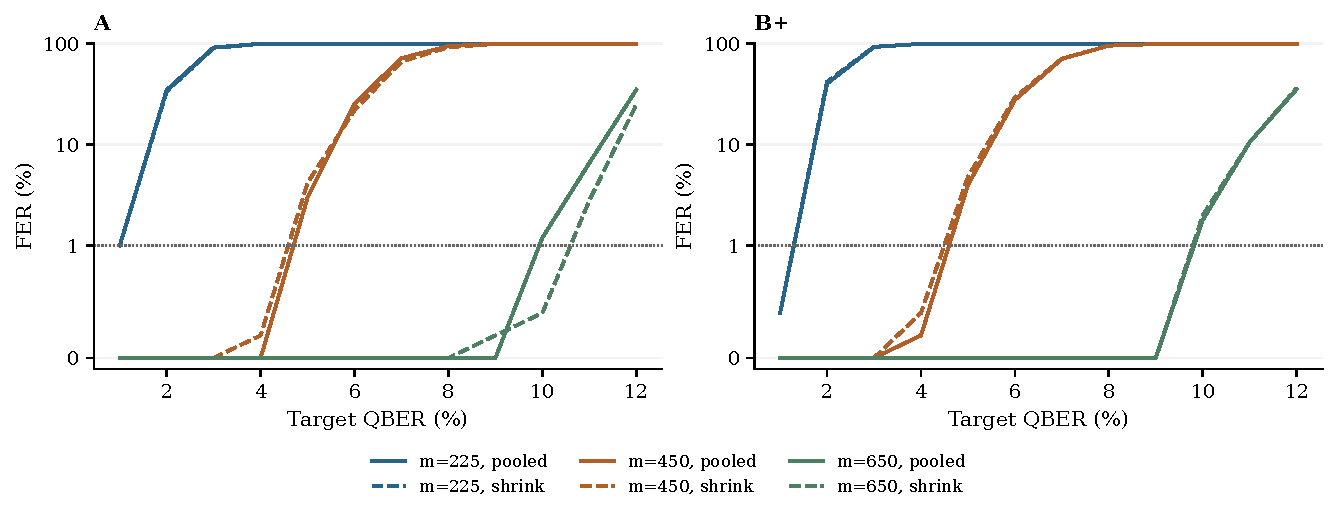
\includegraphics[width=0.94\linewidth]{images/fixed_code_curves.pdf}
\caption{Fixed-code BP curves, with 500 independent frames at each QBER. Solid lines use pooled priors and dashed lines use centred shrinkage. Each color is one matrix, reused across QBER. The dotted line marks 1\% FER; the vertical axis is linear below 1\% and logarithmic above it. Zero observed failures have Wilson 95\% upper bound 0.76\%. Full counts accompany the curves.}
\Description{FER-versus-QBER transitions for three fixed matrices in Scheme A and balanced control B+.}
\label{fig:curves}
\end{figure}

Table~\ref{tab:ablation} compares all four estimators at the same shrinkage-selected
matrix in the 10\% cells. Table~\ref{tab:replication} transfers the frozen row counts to
two fresh matrices and independent frames. Each comparison therefore isolates estimator
or matrix variation without using the evaluation frame to retune the rate.
\begin{table}[htbp]
\centering
\small\setlength{\tabcolsep}{3.2pt}
\caption{Prior-estimation ablation at 10\% QBER. Entries are exact failures out of 2000 paired frames on one common matrix in each cell. P is pooled Jeffreys; J is separate Jeffreys; C is coherent unshrunk; S is centred shrinkage. Complete counts at 2\% and 6\% accompany the same analysis.}
\label{tab:ablation}
\begin{tabular}{@{}llccccc@{}}
\toprule
Encoding & Decoder & $m$ & P & J & C & S \\
\midrule
Standard & BP & 625 & 112 & 10 & 10 & 11 \\
Standard & BP+OSD & 625 & 88 & 6 & 8 & 8 \\
A & BP & 650 & 33 & 13 & 12 & 19 \\
A & BP+OSD & 650 & 28 & 13 & 10 & 13 \\
B & BP & 675 & 3 & 5 & 6 & 4 \\
B & BP+OSD & 675 & 1 & 4 & 5 & 2 \\
B+ & BP & 700 & 0 & 2 & 2 & 1 \\
B+ & BP+OSD & 700 & 0 & 2 & 2 & 1 \\
\bottomrule
\end{tabular}
\end{table}

\begin{table}[htbp]
\centering
\small\setlength{\tabcolsep}{3.2pt}
\caption{Additional matrix seeds at 10\% target QBER. Each seed/encoding uses 1000 fresh frames. Both priors use the shrinkage row count from independent seed-11 calibration. Entries show failure counts, FER percentages, and Wilson 95\% intervals. OSD denotes BP+OSD.}
\label{tab:replication}
\begin{tabular}{@{}clcllll@{}}
\toprule
Seed & Encoding & $m$ & BP P (\%) & BP S (\%) & OSD P (\%) & OSD S (\%) \\
\midrule
29 & Standard & 625 & 62: 6.20 [4.87, 7.87] & 5: 0.50 [0.21, 1.17] & 57: 5.70 [4.43, 7.31] & 4: 0.40 [0.16, 1.02] \\
29 & A & 650 & 17: 1.70 [1.06, 2.71] & 13: 1.30 [0.76, 2.21] & 13: 1.30 [0.76, 2.21] & 11: 1.10 [0.62, 1.96] \\
29 & B+ & 700 & 0: 0.00 [0.00, 0.38] & 1: 0.10 [0.02, 0.56] & 0: 0.00 [0.00, 0.38] & 1: 0.10 [0.02, 0.56] \\
47 & Standard & 625 & 43: 4.30 [3.21, 5.74] & 7: 0.70 [0.34, 1.44] & 36: 3.60 [2.61, 4.94] & 7: 0.70 [0.34, 1.44] \\
47 & A & 650 & 19: 1.90 [1.22, 2.95] & 8: 0.80 [0.41, 1.57] & 12: 1.20 [0.69, 2.09] & 7: 0.70 [0.34, 1.44] \\
47 & B+ & 700 & 0: 0.00 [0.00, 0.38] & 1: 0.10 [0.02, 0.56] & 0: 0.00 [0.00, 0.38] & 1: 0.10 [0.02, 0.56] \\
\bottomrule
\end{tabular}
\end{table}



\FloatBarrier
Table~\ref{tab:channel} retains the same gate-only calibrated matrices while an independent
isotropic channel replaces gate noise at fixed total QBER. The zero-channel row reuses
main holdout frames. The adaptive channel-policy analysis and paired uncertainty are
provided in the computational supplement.

\subsection{A basis-independent channel attenuates the signal}
We insert an independent depolarizing link between preparation and reception, with bit-error
probability $c$ in either basis. Isotropy allows this channel to be commuted to the end of
the path for calculation. The resulting basis probabilities are
\begin{equation}
 p_z^{\mathrm{tot}}=c+(1-2c)p_z^{\mathrm{gate}},\qquad z\in\{r,d\}.
 \label{eq:channel}
\end{equation}
At fixed total QBER $Q$, the average gate contribution is $(Q-c)/(1-2c)$. Increasing $c$
therefore reduces the basis contrast, reaching zero at $c=Q$. This control isolates noise
composition from an increase in overall decoding difficulty.

The link-noise control also narrows the mechanism. At fixed 10\% total QBER and
fixed disclosure, replacing gate noise with isotropic channel noise removes the basis
contrast. At the pure-channel endpoint, the shrinkage and pooled decoders fail on 110 and 98 frames, respectively,
in Standard, and on 33 and 27 in A (Table~\ref{tab:channel}). This fixed-code sensitivity analysis demonstrates
why an estimate of basis contrast can become a liability when that contrast disappears.

\begin{table}[!htbp]
\centering
\small\setlength{\tabcolsep}{3.2pt}
\caption{Fixed-code channel-composition BP controls at 10\% total target QBER. Each cell has 2000 independent holdout frames. The zero-channel points reuse the main cohort. FER entries show counts, percentages, and Wilson 95\% intervals.}
\label{tab:channel}
\begin{tabular}{@{}lcc ll@{}}
\toprule
Encoding & $c$ (\%) & $m$ & FER P (\%) & FER S (\%) \\
\midrule
Standard & 0.0 & 625 & 112: 5.60 [4.67, 6.70] & 11: 0.55 [0.31, 0.98] \\
Standard & 2.5 & 625 & 98: 4.90 [4.04, 5.94] & 31: 1.55 [1.09, 2.19] \\
Standard & 5.0 & 625 & 105: 5.25 [4.36, 6.32] & 86: 4.30 [3.50, 5.28] \\
Standard & 7.5 & 625 & 94: 4.70 [3.86, 5.72] & 93: 4.65 [3.81, 5.66] \\
Standard & 10.0 & 625 & 98: 4.90 [4.04, 5.94] & 110: 5.50 [4.58, 6.59] \\
A & 0.0 & 650 & 33: 1.65 [1.18, 2.31] & 19: 0.95 [0.61, 1.48] \\
A & 2.5 & 650 & 26: 1.30 [0.89, 1.90] & 24: 1.20 [0.81, 1.78] \\
A & 5.0 & 650 & 23: 1.15 [0.77, 1.72] & 24: 1.20 [0.81, 1.78] \\
A & 7.5 & 650 & 25: 1.25 [0.85, 1.84] & 27: 1.35 [0.93, 1.96] \\
A & 10.0 & 650 & 27: 1.35 [0.93, 1.96] & 33: 1.65 [1.18, 2.31] \\
\bottomrule
\end{tabular}
\end{table}
% The lookup rule and rate policies are fixed before evaluation.
\section{Conditional Information, Pooling and Transfer}
\label{app:rule}
\subsection{Information benchmarks}\label{app:information}
For asymptotically reliable one-way reconciliation with known channel probabilities,
conditional entropy supplies the classical benchmark~\cite{slepian1973,elkouss2011}.
The information made available by retaining the basis is
\begin{equation}
 G=H(A\mid B)-H(A\mid B,Z)=I(A;Z\mid B)\geq0.
 \label{eq:information}
\end{equation}
For basis-conditioned binary symmetric channels (BSCs),
\begin{equation}
 H(A\mid B,Z)=\sum_z P(Z=z)h_2(p_z),\qquad
 G=h_2(Q)-\sum_z P(Z=z)h_2(p_z).
 \label{eq:mixtureentropy}
\end{equation}
These are established information identities, not predictions of finite-length BP
performance. The BSC reduction is inappropriate when error probabilities depend
on Alice's bit; then we compute both entropies from the full transition law.

There is also a distinction between knowing the basis and using the full channel.
For error bit $U=A\oplus B$, a basis-only Bernoulli prior has ideal expected
log loss $H(U\mid Z)$, whereas a transition-aware prior can attain
$H(U\mid B,Z)=H(A\mid B,Z)$. Their difference
$D_B=I(U;B\mid Z)$ measures the additional information in Bob's local bit after
conditioning on basis. It is distinct from $G$, whose comparator already uses $B$.
In an asymmetric channel, observing $B=0$ or $B=1$ can change the probability
that a position is erroneous even at fixed $Z$. Thus asymmetric readout can
have $D_B>0$ while $G=0$; thermal relaxation can provide both kinds of information.
These are population log-loss opportunities, not guaranteed finite-sample yield gains.
Neither quantity establishes what an eavesdropper learns.

% BEGIN GENERATED INFORMATION_TABLE
\begin{table}[!htbp]
\centering
\small\setlength{\tabcolsep}{4pt}
\caption{Channel information for the five B+ controls matched to $Q=6\%$. Values are bits per retained bit, computed from the stored transition probabilities with uniform input bits and bases. $G=I(A;Z\mid B)$ is the basis benefit relative to a decoder already using $B$; $D_B=I(U;B\mid Z)$ is the extra ideal error-prior log-loss reduction from Bob\textquotesingle s bit after conditioning on basis. These are distinct quantities and are not added together.}
\label{tab:information}
\begin{tabular}{@{}lrrrr@{}}
\toprule
Mechanism & $H(A\mid B)$ & $H(A\mid B,Z)$ & $G$ & $D_B$ \\
\midrule
Homogeneous & 0.32744 & 0.32744 & 0.00000 & 0.00000 \\
Gate-dependent & 0.32705 & 0.30538 & 0.02166 & 0.00088 \\
Pauli link & 0.32744 & 0.30977 & 0.01768 & 0.00000 \\
Thermal & 0.29886 & 0.29257 & 0.00629 & 0.03274 \\
Readout & 0.29758 & 0.29758 & 0.00000 & 0.02986 \\
\bottomrule
\end{tabular}
\end{table}
% END GENERATED INFORMATION_TABLE


The matched physical controls distinguish basis information from local-bit
information at fixed QBER. Gate-dependent and Pauli noise provide a basis
benefit; readout supplies local-bit information even when the basis benefit
vanishes. Thermal relaxation supplies both. The transition-aware priors in
Appendix~\ref{app:physical} test these differences using finite disclosed samples.

\subsection{Prior estimation and a sample-only pooling rule}
\label{app:reconmethods}
\label{sec:methods}
Let $E_z$ errors be observed among $S_z$ disclosed bits in basis $z$, with
$E=E_r+E_d$ and $S=S_r+S_d$. Define
\begin{equation}
 \widehat p=\frac{E+1/2}{S+1},\qquad
 \widetilde p=\frac ES,\qquad
 \widetilde p_z=\frac{E_z}{S_z}.
 \label{eq:pool}
\end{equation}
Separate Jeffreys estimates introduce a total of one pseudo-error across two classes,
whereas the pooled estimate introduces one half. To avoid crediting extra smoothing to
basis information, our main family retains one common centre:
\begin{equation}
 \widehat p_z(\lambda)=\widehat p+\lambda(\widetilde p_z-\widetilde p),
 \qquad 0\leq\lambda\leq1.
 \label{eq:shrink}
\end{equation}
Its sample-weighted mean is $\widehat p$ before clipping. We call $\lambda=0$ pooled
and $\lambda=1$ coherent separate estimation. An absent class takes the pooled raw
proportion. The positive-part shrinkage comparator uses
\begin{equation}
 d=\widetilde p_d-\widetilde p_r,\quad
 v=\widehat p(1-\widehat p)(S_r^{-1}+S_d^{-1}),\quad
 \lambda_{\mathrm{sh}}=\max\{0,1-v/d^2\},
 \label{eq:weight}
\end{equation}
with weight zero when $d=0$ or a class is absent. This is a plug-in heuristic, not a
dominance guarantee. Separate-Jeffreys and coherent-separate ablations in the circuit
study distinguish centring from shrinkage.

The distinct \emph{selected pooling rule} learns a 24-entry lookup table
from development frames. It chooses $\lambda\in\{0,0.25,0.5,0.75,1\}$ from
sample-only features $S,\widehat p,d^2/v$, maximizing a conservative paired-yield
score. The rule is frozen before confirmation. The rule specification below gives
the bins, score, tie handling, and every selected weight. This is a training
heuristic, not a post-selection confidence guarantee.

Bob's error-vector prior is $L_i=\log[(1-\widehat p_{z_i})/\widehat p_{z_i}]$.
The decoder clips probabilities to $[10^{-6},0.499]$. The lower limit avoids infinite
log odds; the upper limit additionally assumes that a bit is more likely correct
than flipped. This is a model restriction, not a numerical necessity. A retained-record
check finds that neither limit is active for any of the 37,500 confirmation frames
or 25,000 distinct physical-control frames, including transition-aware estimates
whose largest raw probability is 0.2572. These results therefore do not test channels
that require negative error-prior log odds. Each frame's sample is disjoint from its decoded bits. Population asymmetry and true error
probabilities are forbidden inputs to the deployed rule. Oracle pooled and oracle
basis priors are reported only as benchmarks for the cost of learning probabilities.

\subsection{Confirmation design}
To vary sample size independently of a circuit-specific contrast, the confirmation study uses
basis-conditioned BSCs with $p_r=Q(1-a)$ and $p_d=Q(1+a)$. Its 75 cells cross
$Q\in\{0.02,0.06,0.10\}$, $a\in\{0,0.1,0.25,0.5,0.75\}$, and
$S\in\{50,100,200,500,1000\}$ at $n=1000$. Independent symmetric reference
calibration uses 450 frames to select $m=250,475,600$ at the three QBERs, respectively,
near a 10\% FER transition. A 15,000-frame pilot learns the pooling table on matrix
seed 11. Confirmation uses 37,500 new frames and unseen matrix seed 29, with 500
frames per cell, but retains the pilot's entire $(Q,a,S)$ grid and the same $m$
values. It therefore tests replication within the development design, not generalization
to new conditions or code families. The transfer experiment in
Section~\ref{sec:transfer} supplies that distinct test. These sensitivity conditions
also differ from the circuit study's low-FER operating points.

\subsection{Unseen codes, longer blocks, and fixed resources}
Transfer uses a three-partition Gallager construction and an irregular construction with
the variable-degree fractions of Elkouss et al.~\cite{elkouss2009}, converted from edge
to node fractions. A bounded local-cycle search and degree-balanced checks realize the
latter. Its check distribution differs from the published ensemble, and row fractions
above 0.50 reuse the 0.50 variable-degree profile. No published asymptotic threshold or
state-of-the-art efficiency is attributed to these realizations.

Development libraries use seeds 101 and 103 at $n=1000,4000,16000$; five unseen
libraries use seeds 211, 223, 227, 229, and 233. All confirmation and transfer/control
decoders use layered sum-product BP with 100 sweeps and the same verification rule.
OSD is evaluated only in the circuit study. The selected prior and the transfer policies
are not claimed to retain their effects under an OSD retry.

Two complementary comparisons are retained. A fixed-code comparison uses one common
matrix and disclosure, chosen to maximize pooled-decoder yield on independent 6\%-QBER
development data spanning $a=0,0.5$ and $S=50,200,1000$. A pipeline comparison lets
each method choose its syndrome length from the same row-fraction pool, 0.15 to 0.80
in steps of 0.05. Both use the same sample features, ridge-logistic training procedure,
and development budget to predict FER and maximize expected $Y$ before decoding.
Development evaluates entropy-margin subsets of this pool; predictions for some
feature/rate combinations therefore extrapolate beyond training support. The policies
are comparable learned selectors, not globally optimal rate adaptation.

At $Q=0.06$, transfer crosses the three block lengths with
$(a,S)=(0,50),(0.25,200),(0.75,1000)$. Asymmetry and sample size vary together,
so this transfer design does not estimate their separate effects or test unseen QBERs. A pilot-based precision calculation selects
500 paired frames per matrix and condition. A separate fixed-total experiment keeps
$n+S=2000$, $Q=0.06$, and $a=0.5$, transfers the policies without retuning, and
constructs matrices at the exact retained length $n=2000-S$. No padded bits are
counted as data. Physical controls use B+ at $n=1000,S=200$ with five noise
mechanisms, both at fixed parameters and after matching the overall QBER to 6\%.
Their transition laws and the Bob-bit-conditioned prior are specified in
Appendix~\ref{app:physical}.

\subsection{Frozen pooling rule}

Table~\ref{tab:rule} gives every weight in the frozen lookup rule. The lower sample bin
includes $S=100$; a QBER or squared-contrast value exactly at a cut point enters the
upper bin. All bin inputs come from the current frame's disclosed sample. Weights were
selected on 15,000 pilot frames and were not retuned on the 37,500 confirmation frames
or any transfer/control outcomes. The pilot score selects among five weights within
each bin. For the $N_b$ pilot frames assigned to bin $b$, let
$\Delta_i(\lambda)=Y_i(\lambda)-Y_i(0)$ be the paired yield difference, using
the same frame and code for both weights and the yield in Eq.~\eqref{eq:yield}.
For $N_b>1$, the selection score is
\begin{equation}
 L_b(\lambda)=\overline\Delta_b(\lambda)
 -1.96\sqrt{\frac{\sum_{i\in b}[\Delta_i(\lambda)-\overline\Delta_b(\lambda)]^2}
 {N_b(N_b-1)}}.
 \label{eq:poolingscore}
\end{equation}
This uses the sample standard deviation of paired differences divided by
$\sqrt{N_b}$. The chosen weight maximizes $L_b$ over the ascending grid
$(0,0.25,0.5,0.75,1)$; exact ties choose the smallest weight. For $N_b\leq1$
all scores are set to zero, selecting pooling. The 1.96 penalty is a development
heuristic, not a simultaneous or post-selection confidence guarantee.
The implementation is \texttt{extensions/pilot.py}, function \texttt{train},
under \texttt{supplementary/}; the stored rule retains every bin count and score.

% BEGIN GENERATED RULE_TABLE
\begin{table}[!htbp]
\centering
\small\setlength{\tabcolsep}{4pt}
\caption{Frozen partial-pooling weights $\lambda$ selected using pilot data only. Columns give the squared sample contrast $d^2/v$.}
\label{tab:rule}
\begin{tabular}{@{}llrrrr@{}}
\toprule
Sample & Pooled estimate & $<1$ & $[1,4)$ & $[4,9)$ & $\geq9$ \\
\midrule
$S\leq100$ & $\widehat p<0.04$ & 0.25 & 0.25 & 0 & 0 \\
$S\leq100$ & $0.04\leq\widehat p<0.08$ & 0 & 0.25 & 0.25 & 0 \\
$S\leq100$ & $\widehat p\geq0.08$ & 0 & 0.5 & 0.5 & 0.5 \\
$S>100$ & $\widehat p<0.04$ & 0 & 0.5 & 0.5 & 1 \\
$S>100$ & $0.04\leq\widehat p<0.08$ & 0 & 0 & 0.75 & 0.75 \\
$S>100$ & $\widehat p\geq0.08$ & 0 & 0.5 & 0.5 & 0.75 \\
\bottomrule
\end{tabular}
\end{table}
% END GENERATED RULE_TABLE

The transfer policies use nine standardized features: pooled entropy, pooled QBER,
$\log(1+\min\{100,d^2/v\})$, $S^{-1/2}$, $\log(n/1000)$, row fraction
$\beta=m/n$, $\beta-h_2(\widehat p)$, its square, and pooled entropy times the
log-contrast feature. Each family/prior has a logistic FER model with an unpenalized
intercept and ridge coefficient one for every other standardized coefficient.
Development crosses three QBERs, two asymmetries, three sample sizes, three lengths,
and two library seeds, with 100 input frames per condition. Candidate row fractions
are the shared-pool values nearest $\alpha h_2(Q)$ for
$\alpha\in\{1.1,1.35,1.6,1.9\}$. Generator $Q$ defines this development design;
the deployed features use sampled $\widehat p$. The model then predicts every
candidate in the full row-fraction pool before choosing a test-frame code.

This development design produces 10,800 independent input frames. The other cohorts
comprise 15,000 pilot, 37,500 confirmation, 22,500 transfer,
12,500 fixed-total, and 25,000 physical-control frames, for 123,300 in total.
Matching inputs across families, methods, or candidate rates are counted once.
The 450 reference-calibration frames are additional. Reusing the input frames across
decoders and policies produces 1,163,400 outputs; the diagnostic reference-and-stress cohort
contains 45,000 acquisition replicate blocks. Basis/range and held-out validation
add 31,000 blocks. Full-observation validation adds 6500 blocks; its target-profile
analysis reuses 2500 fitting records from held-out validation. Acquisition counts
and reuse rules are specified in Appendix~\ref{app:diagnostic}.

\subsection{Complete confirmation results}
\label{app:confirmation}
The table and heatmap retain all 75 confirmation conditions and every comparator.
The selected rule's worst cell, at $Q=2\%,a=0.1,S=200$, has nine harmed
and no rescued frames: a -1.029 pp yield difference with Holm-adjusted
$p=0.180$. Its equal-cell mean gain is 0.813 pp, compared with 1.804 pp
for the oracle basis prior. Both quantities condition on the repeated
development grid and the unseen confirmation matrix.
% BEGIN GENERATED ASYMMETRY_TABLE
\begin{table}[!htbp]
\centering
\small\setlength{\tabcolsep}{4pt}
\caption{Confirmation against estimated pooling. Supported gains and harms pass a two-sided exact McNemar test with Holm correction across 75 cells separately for each method. All cells have 500 paired frames. Means weight cells equally; the equal-basis column uses the 15 cells with $a=0$. Yield differences are in percentage points.}
\label{tab:asymmetry}
\begin{tabular}{@{}lrrrr@{}}
\toprule
Prior & Gains /75 & Harms /75 & Mean $\Delta Y$ & $a=0$ mean \\
\midrule
Coherent separate & 21 & 23 & -0.509 & -2.297 \\
Positive-part shrinkage & 23 & 5 & +0.669 & -0.444 \\
Selected pooling & 25 & 0 & +0.813 & -0.056 \\
Oracle pooled & 6 & 0 & +0.413 & +0.376 \\
Oracle basis & 41 & 0 & +1.804 & +0.376 \\
\bottomrule
\end{tabular}
\end{table}
% END GENERATED ASYMMETRY_TABLE
\begin{figure}[!htbp]
\centering
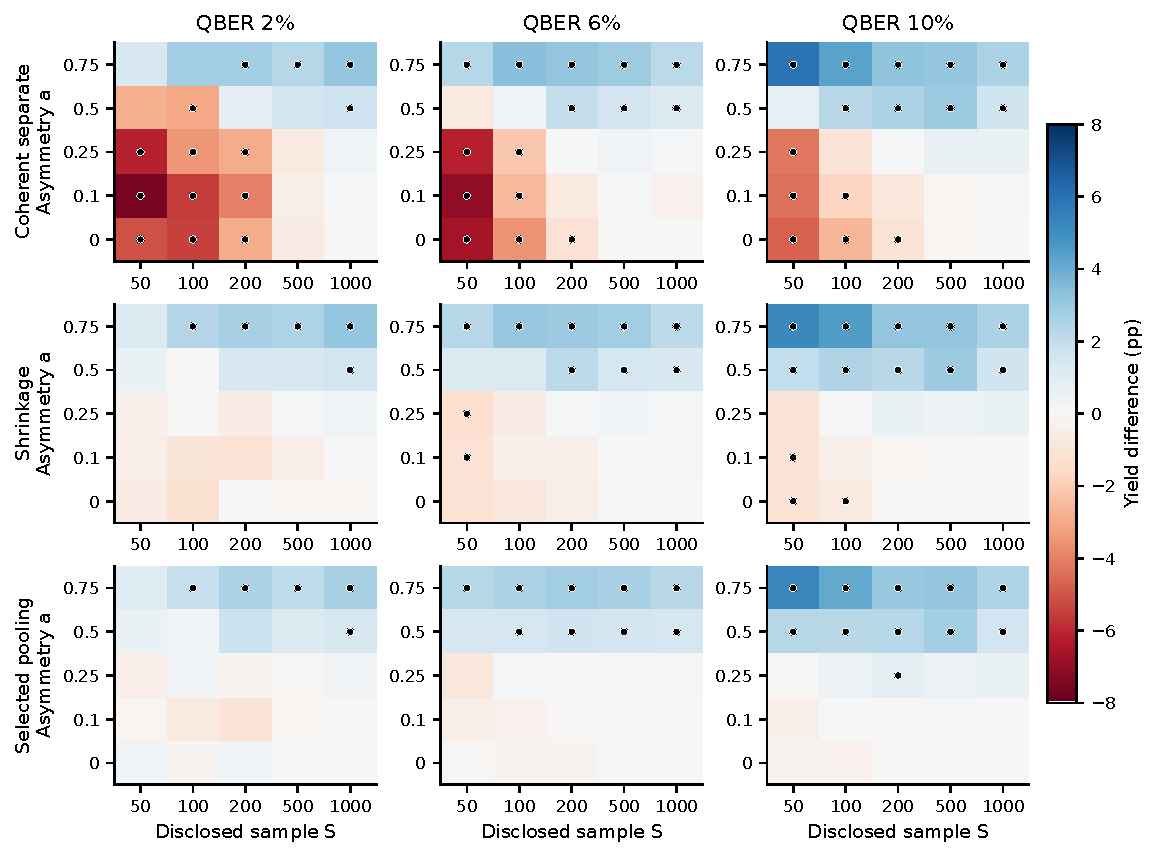
\includegraphics[width=0.98\linewidth]{images/asymmetry_map.pdf}
\caption{Confirmation yield changes relative to estimated pooling, in percentage points.
Rows compare coherent separate estimation, positive-part shrinkage, and the frozen
selected rule; columns give target QBER. Each panel includes all five asymmetries and
sample sizes, with 500 paired frames per cell. A dot marks a two-sided McNemar result
passing Holm correction over 75 cells for that comparator. Colour shows direction and
magnitude, not a confidence bound. Each QBER uses one fixed unseen matrix.}
\Description{Nine heatmaps show that separate estimates can harm weak-contrast cells,
while the selected pooling rule retains many gains and reduces these harms.}
\label{fig:asymmetry}
\end{figure}
\subsection{Transfer accounting and absolute outcomes}
The information benchmark puts these gains in context. At~\mbox{$Q=6\%,a=0.75$},
the pooled and basis-conditioned BSC entropies are 0.32744 and 0.29850 bits per
retained bit, so $G=0.02894$. Neither learned policy approaches those ideal floors:
the selected mean row fractions at $n=16000$ are 0.49330 for Gallager and 0.42520
for the irregular construction. A gain between two finite implementations is
therefore not a direct measure of the fraction of $G$ recovered.

To separate the recorded yield contributions, write $V_j=(n-m_j-64)/(n+S)$ and
$L_j=V_j(1-I_j)$ for each paired method $j\in\{\mathrm P,\mathrm S\}$. Then
\begin{equation}
 Y_{\mathrm S}-Y_{\mathrm P}
 =\underbrace{\frac{m_{\mathrm P}-m_{\mathrm S}}{n+S}}_{D}
 +\underbrace{L_{\mathrm P}-L_{\mathrm S}}_{R}.
 \label{eq:yielddecomposition}
\end{equation}
Here $D$ accounts for fewer syndrome rows and $R$ for the change in yield lost to
failed recovery. This is an exact accounting identity, not a causal attribution to
the prior: the fitted FER model, training variation, extrapolation, and tolerated
failure can all change the selected rows. The strong-asymmetry Gallager gain comprises +0.736 pp from
syndrome length and +0.337 pp from recovery; for the irregular construction these
terms are +4.316 and -0.163 pp (Table~\ref{tab:yieldaccounting}). The latter disclosure gain exceeds the 2.724 pp
difference between ideal entropy-limited yields at this sample fraction because
the implementations have different excess disclosure above their respective floors.
It does not imply an information-theoretic gain larger than the channel provides.


Table~\ref{tab:yieldaccounting} decomposes the longest-block, strong-asymmetry
comparison at the frame level. If $c_{\rm P}=\overline m_{\rm P}/n$ and
$c_{\rm S}=\overline m_{\rm S}/n$, define excess row fractions relative to the BSC
entropy benchmarks by $\epsilon_{\rm P}=c_{\rm P}-h_2(Q)$ and
$\epsilon_{\rm S}=c_{\rm S}-H(A\mid B,Z)$. The identity
$c_{\rm P}-c_{\rm S}=G+\epsilon_{\rm P}-\epsilon_{\rm S}$ separates the difference
of ideal floors from the difference in implementation overhead. The excess includes
code construction, finite samples, rate selection, and tolerated failure; it is not
an independently isolated coding penalty.



% BEGIN GENERATED YIELD_ACCOUNTING_TABLE
\begin{table}[!htbp]
\centering
\small\setlength{\tabcolsep}{4pt}
\caption{Accounting for strong-asymmetry transfer at $n=16000,S=1000,Q=6\%,a=0.75$. Means use the same 2500 frames per family as the transfer comparison. $D$ is the yield change due to syndrome length and $R$ the change in failure-related loss, so $\Delta Y=D+R$. The pooled and conditional entropy benchmarks are 0.32744 and 0.29850 bits per retained bit. $D$, $R$, and $\Delta Y$ are percentage points.}
\label{tab:yieldaccounting}
\begin{tabular}{@{}lrrrrr@{}}
\toprule
Family & $\overline m_{\rm P}/n$ & $\overline m_{\rm S}/n$ & $D$ & $R$ & $\Delta Y$ \\
\midrule
Gallager & 0.50112 & 0.49330 & +0.736 & +0.337 & +1.072 \\
Irregular & 0.47106 & 0.42520 & +4.316 & -0.163 & +4.154 \\
\bottomrule
\end{tabular}
\end{table}
% END GENERATED YIELD_ACCOUNTING_TABLE

% BEGIN GENERATED ABSOLUTE_TRANSFER_TABLE
\begin{table}[!htbp]
\centering
\small\setlength{\tabcolsep}{4pt}
\caption{Absolute pipeline outcomes at $n=16000,Q=6\%$. Each row pools 2500 frames across five libraries. P/S denote pooled/selected priors and their own learned selectors; $S=50$ at $a=0$ and $S=1000$ at $a=0.75$. FER entries give failure counts and percentages; $Y$ is a percentage. Timing is retained parallel-batch wall time divided by frames, in milliseconds; it is not single-frame latency or a controlled hardware benchmark. Full absolute outcomes and uncertainty for every condition accompany the supplement.}
\label{tab:absolutetransfer}
\begin{tabular}{@{}lrrlrrrr@{}}
\toprule
Family & $a$ & Prior & FER & $Y$ & $\overline m/n$ & $f_{\rm EC}$ & ms/frame \\
\midrule
Gallager & 0 & P & 468: 18.72 & 38.60 & 0.48697 & 1.499 & 7.63 \\
Gallager & 0 & S & 469: 18.76 & 38.57 & 0.48697 & 1.499 & 8.06 \\
Gallager & 0.75 & P & 15: 0.60 & 46.24 & 0.50112 & 1.543 & 2.11 \\
Gallager & 0.75 & S & 0: 0.00 & 47.31 & 0.49330 & 1.519 & 1.60 \\
Irregular & 0 & P & 477: 19.08 & 41.09 & 0.45632 & 1.406 & 14.42 \\
Irregular & 0 & S & 485: 19.40 & 42.01 & 0.44004 & 1.356 & 15.02 \\
Irregular & 0.75 & P & 5: 0.20 & 49.29 & 0.47106 & 1.451 & 3.34 \\
Irregular & 0.75 & S & 12: 0.48 & 53.45 & 0.42520 & 1.311 & 4.00 \\
\bottomrule
\end{tabular}
\end{table}
% END GENERATED ABSOLUTE_TRANSFER_TABLE

Table~\ref{tab:transferall} gives every numerical comparison behind Figure~\ref{fig:transfer}.
Its five-library intervals do not include variation from retraining the development
policies or choosing a different code ensemble.

% BEGIN GENERATED TRANSFER_TABLE
\begin{table}[htbp]
\centering
\small\setlength{\tabcolsep}{4pt}
\caption{All transfer conditions at 6\% QBER. Paired yield differences in percentage points, with exploratory 95\% $t_4$ intervals across five matrix libraries. Fixed-code comparisons hold code and disclosure constant; pipeline comparisons include the separately trained rate selectors.}
\label{tab:transferall}
\begin{tabular}{@{}lrrrll@{}}
\toprule
Family & $n$ & $a$ & $S$ & Fixed code [95\% CI] & Pipeline [95\% CI] \\
\midrule
Gallager & 1000 & 0 & 50 & -0.10 [-0.19, -0.01] & -0.40 [-0.69, -0.11] \\
Gallager & 1000 & 0.25 & 200 & +0.00 [+0.00, +0.00] & -0.15 [-0.35, +0.05] \\
Gallager & 1000 & 0.75 & 1000 & +0.19 [+0.11, +0.27] & +1.08 [+0.73, +1.43] \\
Gallager & 4000 & 0 & 50 & -0.72 [-1.03, -0.40] & -0.64 [-0.90, -0.38] \\
Gallager & 4000 & 0.25 & 200 & +0.00 [-0.09, +0.09] & +0.09 [-0.04, +0.22] \\
Gallager & 4000 & 0.75 & 1000 & +0.70 [+0.51, +0.89] & +0.83 [+0.69, +0.96] \\
Gallager & 16000 & 0 & 50 & -0.09 [-0.20, +0.03] & -0.02 [-0.09, +0.04] \\
Gallager & 16000 & 0.25 & 200 & +0.00 [+0.00, +0.00] & +0.17 [-0.06, +0.41] \\
Gallager & 16000 & 0.75 & 1000 & +0.00 [+0.00, +0.00] & +1.07 [+0.91, +1.24] \\
Irregular & 1000 & 0 & 50 & -0.11 [-0.30, +0.08] & -0.18 [-0.66, +0.29] \\
Irregular & 1000 & 0.25 & 200 & +0.02 [-0.07, +0.10] & +0.18 [+0.04, +0.33] \\
Irregular & 1000 & 0.75 & 1000 & +0.38 [+0.05, +0.71] & +1.49 [+1.09, +1.89] \\
Irregular & 4000 & 0 & 50 & +0.02 [-0.04, +0.08] & +1.16 [+0.78, +1.55] \\
Irregular & 4000 & 0.25 & 200 & +0.04 [-0.03, +0.11] & +0.05 [-0.06, +0.17] \\
Irregular & 4000 & 0.75 & 1000 & +0.19 [-0.15, +0.53] & +3.55 [+3.25, +3.85] \\
Irregular & 16000 & 0 & 50 & +0.00 [-0.10, +0.10] & +0.92 [+0.60, +1.23] \\
Irregular & 16000 & 0.25 & 200 & +0.00 [+0.00, +0.00] & -0.06 [-0.59, +0.47] \\
Irregular & 16000 & 0.75 & 1000 & +0.08 [-0.15, +0.31] & +4.15 [+3.94, +4.37] \\
\bottomrule
\end{tabular}
\end{table}
% END GENERATED TRANSFER_TABLE
% BEGIN GENERATED SAMPLE_TABLE
\begin{table}[!htbp]
\centering
\small\setlength{\tabcolsep}{4pt}
\caption{Fixed total of 2000 sifted bits, at $Q=6\%$ and $a=0.5$. Yields are percentages; differences are percentage points with exploratory 95\% intervals across five matrix libraries, each with 500 paired frames. Policies are transferred without retuning on these outcomes.}
\label{tab:sample}
\begin{tabular}{@{}lrrrrl@{}}
\toprule
Family & $S$ & $n$ & Pooled $Y$ & Selected $Y$ & $\Delta Y$ [95\% CI] \\
\midrule
Gallager & 50 & 1950 & 36.81 & 36.75 & -0.05 [-0.47, +0.36] \\
Gallager & 100 & 1900 & 37.42 & 38.25 & +0.83 [+0.50, +1.17] \\
Gallager & 200 & 1800 & 37.62 & 38.33 & +0.71 [+0.47, +0.95] \\
Gallager & 500 & 1500 & 32.95 & 33.47 & +0.53 [+0.30, +0.75] \\
Gallager & 1000 & 1000 & 20.68 & 21.24 & +0.56 [+0.30, +0.82] \\
Irregular & 50 & 1950 & 37.44 & 39.18 & +1.74 [+1.12, +2.36] \\
Irregular & 100 & 1900 & 40.21 & 41.18 & +0.97 [+0.82, +1.13] \\
Irregular & 200 & 1800 & 41.15 & 42.27 & +1.12 [+0.87, +1.38] \\
Irregular & 500 & 1500 & 35.49 & 36.75 & +1.27 [+0.93, +1.60] \\
Irregular & 1000 & 1000 & 22.63 & 23.46 & +0.83 [+0.65, +1.02] \\
\bottomrule
\end{tabular}
\end{table}
% END GENERATED SAMPLE_TABLE

\FloatBarrier
% Physical controls use observable inputs and the same disclosed sample.
\section{Physical Transition Controls}
\label{app:physical}
B+ uses two Alice operations and one Bob operation for each complete path. We evaluate
one noise mechanism at a time: homogeneous depolarization $p=0.03$ per operation;
gate-dependent depolarization $(p_X,p_H,p_I)=(0.02,0.05,0.005)$; a Pauli link
with $(p_X,p_Y,p_Z)=(0.015,0.005,0.075)$; thermal relaxation with
$T_1=1800$ ns, $T_2=2500$ ns and operation durations $(40,60,50)$ ns for
$(X,H,I)$; and readout errors $(0\to1,1\to0)=(0.01,0.11)$.
Non-selected mechanisms are ideal. Fixed-parameter comparisons retain these values;
matched comparisons scale the probabilities or durations by a common factor until
overall QBER equals 0.06. The values specify controlled simulations, not fitted hardware.
The thermal parameters satisfy $T_2\leq2T_1$.

Let $t_{z,01}=\Pr(B=1\mid A=0,Z=z)$ and
$t_{z,10}=\Pr(B=0\mid A=1,Z=z)$. Jeffreys-smoothed sample counts estimate each
transition separately. Under the uniform Alice prior, the transition-aware error prior is
\begin{equation}
 \widehat p_{z,B=0}=\frac{\widehat t_{z,10}}
 {1-\widehat t_{z,01}+\widehat t_{z,10}},\qquad
 \widehat p_{z,B=1}=\frac{\widehat t_{z,01}}
 {1-\widehat t_{z,10}+\widehat t_{z,01}}.
\end{equation}
These probabilities use Bob's own measured bit and the disclosed sample. The same
numerical clipping as for the basis priors is applied. An observable-input perturbation
audit changes population parameters and undisclosed Alice/error bits while holding Bob's
word fixed; deployed priors and selection features remain unchanged.

For a transition pair $(t_{01},t_{10})$ and uniform Alice bits,
\begin{equation}
 H(A\mid B)=1+\tfrac12[h_2(t_{01})+h_2(t_{10})]
 -h_2\!\left(\tfrac{1+t_{01}-t_{10}}2\right).
\end{equation}
Applying this expression to the pooled pair gives $H(A\mid B)$; averaging its
per-basis values gives $H(A\mid B,Z)$. Direct summation of the full joint
probabilities independently checks both calculations. Table~\ref{tab:information}
reports these benchmarks for the same transition laws used in decoding.


Table~\ref{tab:physical} reports every matched-QBER comparison. Fixed-parameter
controls and all prior ablations accompany the computational supplement.

% BEGIN GENERATED PHYSICAL_TABLE
\begin{table}[!htbp]
\centering
\small\setlength{\tabcolsep}{4pt}
\caption{B+ physical controls matched to 6\% overall QBER. Paired yield differences from estimated pooling are in percentage points, with exploratory 95\% $t_4$ intervals across five libraries (500 frames each). Both compared priors use the same fixed code and disclosure as pooling. Selected uses basis; transition-aware also uses Bob\textquotesingle s local bit.}
\label{tab:physical}
\begin{tabular}{@{}llll@{}}
\toprule
Mechanism & Family & Selected [95\% CI] & Transition-aware [95\% CI] \\
\midrule
Homogeneous & Gallager & -0.01 [-0.05, +0.03] & -0.70 [-0.87, -0.52] \\
Homogeneous & Irregular & -0.03 [-0.09, +0.02] & -0.63 [-0.95, -0.32] \\
Gate-dependent & Gallager & +0.25 [+0.11, +0.38] & +0.17 [-0.02, +0.37] \\
Gate-dependent & Irregular & +0.37 [+0.16, +0.58] & +0.42 [+0.22, +0.63] \\
Pauli link & Gallager & +0.20 [-0.10, +0.51] & +0.17 [-0.02, +0.37] \\
Pauli link & Irregular & +0.31 [+0.22, +0.39] & +0.40 [+0.23, +0.58] \\
Thermal & Gallager & -0.04 [-0.09, +0.01] & +0.32 [+0.04, +0.59] \\
Thermal & Irregular & +0.06 [-0.07, +0.20] & +0.58 [+0.18, +0.99] \\
Readout & Gallager & -0.03 [-0.11, +0.05] & +0.29 [+0.23, +0.35] \\
Readout & Irregular & -0.03 [-0.18, +0.12] & +0.53 [+0.15, +0.91] \\
\bottomrule
\end{tabular}
\end{table}
% END GENERATED PHYSICAL_TABLE

The Gallager transition-aware entries for gate-dependent and Pauli noise have the
same mean and interval because their net rescued-frame counts across the five
libraries are $(6,1,1,3,1)$ and $(6,3,1,1,1)$, respectively. The different frame
outcomes give the same unordered set of matrix-level gains, hence the same $t_4$
summary.

\FloatBarrier
% The target depends on which devices are scaled during acquisition.
\section{Separated-Device Response and Fitting}
\label{app:diagnostic}
For Standard basis $b\in\{0,1\}$ and bit $x\in\{0,1\}$, define
\begin{align}
 a_{bx}&=\frac{1-(1-p_A)^{x+b}(1-p_B)^b}{2}, &
 q_0(p_A,p_B)&=\frac14\sum_{b,x}a_{bx},\\
 u_{bx}&=\frac{1-(1-p_A)^{x+b}(1-p_E)^b}{2}, &
 v_{bx}&=\frac{1-(1-p_E)^{x+b}(1-p_B)^b}{2}.
\end{align}
Conditioning on Eve's basis and measurement outcome gives
\begin{equation}
 q_I(p_A,p_B,p_E)=\frac14+\frac18\sum_{b,x}
 \big[(1-u_{bx})v_{bx}+u_{bx}(1-v_{b,1-x})\big].
 \label{eq:twohop}
\end{equation}
The $1/4$ term comes from the random-basis mismatch branch. The remaining term
averages the two noisy hops in the matching branch, including the changed state resent
after an erroneous Eve measurement. Direct density-state propagation checks the formula.
Setting $p_E=0$ yields the ideal-Eve identity used for calibrated inversion in the text.

For $E_j$ errors among $N_j$ sifted measurements, fits use $y_j=E_j/N_j$ and
weights $1/\widehat V_j$, where
$\widehat V_j=u_j(1-u_j)/N_j$ and $u_j=(E_j+1/2)/(N_j+1)$.
The gate fit minimizes weighted squared residuals, profiling the affine parameter $r$
at every candidate $p$. Bounds are
$10^{-8}\leq p\leq\min(0.3,0.999/\max f)$ and $-0.5\leq r\leq1.5$.
Allowing signed $r$ avoids truncating point estimates at zero, but the optimization is
not unconstrained. Local inverse-information and delta-method standard errors produce
intervals $\widehat e\pm1.959964\,\widehat{\mathrm{SE}}$ without endpoint clipping.
Boundary and finite-count coverage failures are retained.

With $J_j=\nabla_{(p,r)}Q_{f_j}$ and expected sifted allocation $N_j=T_j/2$,
the design information is
$F=\sum_j N_jJ_jJ_j^{\mathsf T}/[Q_{f_j}(1-Q_{f_j})]$.
The reference-and-stress design minimizes the worst $(F^{-1})_{rr}/16$ over the declared
$(p,r)$ grid. Candidate high scales are 2.5, 4, 6, and 8; low-scale shares are
0.5, 0.6, 0.7, 0.8, and 0.9. Calibration shares range from 0.2 to 0.8 in
steps of 0.1 and use a corresponding delta-variance objective. Selection precedes
all diagnostic Monte Carlo acquisitions.

\subsection{Acquisition records and basis/range validation}
\label{app:range}
Held-out prediction is a check on an additional response setting, not directly
on the extrapolated residual. In the unequal-noise case $(p_A,p_B,r)=(0.01,0.05,0.2)$,
the basis fit covers the held-out response in 92.8\% of replicates while its
residual interval covers in 87.8\%. This contrast motivates the target-specific
profile analysis below.

The observation hierarchy is aggregate QBER, two basis rates, and four
bit-and-basis transition rates. The full operating acquisition draws stratum
counts from $\mathrm{Multinomial}(T;1/8,1/8,1/8,1/8,1/2)$, with the final category
discarded. Conditional errors are binomial with the path probabilities in
Eq.~\eqref{eq:attack}. Scaling instead draws a sifted count
$N_j\sim\mathrm{Binomial}(T_j,1/2)$ and aggregate errors at each setting.
Different acquisition strategies use independent records; estimators of a given
operating acquisition reuse its exact counts. The cross-circuit study has 6500
replicate blocks: nine circuit/device cells, three Standard readout cells, and
one Standard zero-interception cell, each with 500 replicates and two fully
budgeted acquisitions. No observations used for inference are key producing.
At unscaled readout probability $c=0.01$, the full Standard estimator's
coverage is 93.8--94.8\% for the combined residual $e_c$, but only
74.2--74.6\% for the interception-only target. These readout cells use the
same three device pairs as the main cross-circuit comparison. The changed
coverage illustrates target confounding rather than loss of identification
of the combined disturbance.



For a single basis-resolved acquisition, the two matched counts and the discarded
count follow a multinomial law with probabilities $(1/4,1/4,1/2)$. Conditional
error counts are binomial with rates from Eq.~\eqref{eq:basis}. The
constrained basis fit profiles the affine interception parameter; the direct
inverse uses the same observed proportions without projecting its parameter
estimates. An inverse is marked unavailable if a basis count is zero,
$|1-2\widehat Q_r|\leq10^{-12}$, or the square-root discriminant is at most
$10^{-12}$. Other finite real inverses are retained without projection. All
31,000 basis records pass these checks. An empty rectilinear-zero subset has no
point estimate and the interval $[0,1]$; none occurs in the cross-circuit records. Scaling and
calibration acquisitions use independent transmitted signals for each declared
allocation; all setting allocations sum to the strategy's budget.

The matched-range design minimizes the worst residual Fisher variance over all
16 nominal $(p,r)$ pairs at $T=8000$, using expected sifted counts $N_j=4000w_j$.
For each cap $c\in\{2.5,4,8\}$, the two-setting design fixes $(1,c)$.
Four-setting designs fix both endpoints and choose any two of the five interior
points $1+j(c-1)/6$, $j=1,\ldots,5$, in increasing order. Every allocation is
$w_j=u_j/20$ with positive integer $u_j$ and $\sum_j u_j=20$: 19 allocations
for two settings and 969 for each of the ten four-setting location sets.
Allocations and location pairs are enumerated lexicographically; the first minimum
allocation is retained. A location set replaces the incumbent only when its
objective improves by more than $10^{-15}$. The exact configuration and enumeration
are \texttt{diagnostic\_validation/protocol.json} and function
\texttt{configurations} in \texttt{diagnostic\_validation/experiment.py}, under
\texttt{supplementary/}. The selected
low-setting shares for two-setting designs are 65\%, 70\%, and 75\% at caps
2.5, 4, and 8. Four-setting choices, with weights in the same order, are
\begin{align*}
 f&=(1,1.25,2.25,2.5), & w&=(0.60,0.05,0.05,0.30),\\
 f&=(1,3,3.5,4), & w&=(0.70,0.05,0.05,0.20),\\
 f&=(1,17/3,41/6,8), & w&=(0.75,0.05,0.05,0.15).
\end{align*}
These designs are frozen before the 28,500 nominal/interpolation replicate blocks.
Their eight strategies comprise 228,000 budgeted acquisitions. The basis inverse
is an additional estimator, not an additional acquisition. The supplement gives
all 513 estimator/cell summaries, including Monte Carlo intervals. For a
fixed-grid mean, independent cell variances are summed and divided by the square
of the number of cells; differences use paired estimator errors when counts are
shared and independently sampled errors otherwise.

For calibration proportions $\widehat h$ and $\widehat Q$, the gate-model estimate is
\begin{equation}
 \widehat e_{\mathrm{gate}}=
 q_I(0,0,p_E)\frac{\widehat Q-q_0(\widehat p,\widehat p)}
 {q_I(\widehat p,\widehat p,p_E)-q_0(\widehat p,\widehat p)},
 \qquad q_0(\widehat p,\widehat p)=\widehat h.
 \label{eq:calgate}
\end{equation}
With ideal Eve, $q_I(p_A,p_B,0)=1/4+q_0(p_A,p_B)/2$, so this reduces exactly
to the calibrated BSC expression $(\widehat Q-\widehat h)/(1-2\widehat h)$.
The two names denote one estimator in this comparison. A separate reference-and-stress
cohort includes linear extrapolation and the Fiorini interception-density
formula~\cite{fiorini2026}, with all outcomes retained in the supplement.


% BEGIN GENERATED VALIDATION_TABLE
\begin{table}[!htbp]
\centering
\small\setlength{\tabcolsep}{4pt}
\caption{Diagnostic validation, with 500 replicates per cell. Nominal means weight 48 cells equally; interpolation means weight nine interior cells at $T=8000$. MAE and its 95\% Monte Carlo (MC) interval are in percentage points (pp). Coverage is the average percentage of individual nominal 95\% intervals covering the target, shown as nominal/interpolation. The two basis estimators reuse the same counts. Intervals condition on the frozen grids and do not establish equivalence.}
\label{tab:validation}
\begin{tabular}{@{}lllr@{}}
\toprule
Estimation/acquisition & Nominal MAE [MC CI] & Interpolation MAE [MC CI] & Cover. (\%) \\
\midrule
Basis, constrained fit & 0.504 [0.498, 0.510] & 0.461 [0.450, 0.471] & 95.3/95.7 \\
Basis, direct inverse & 0.534 [0.528, 0.540] & 0.468 [0.458, 0.479] & 94.8/95.4 \\
Two settings, $f_{\max}=2.5$ & 0.817 [0.808, 0.827] & 0.755 [0.738, 0.772] & 96.0/95.4 \\
Four settings, $f_{\max}=2.5$ & 0.853 [0.843, 0.863] & 0.748 [0.731, 0.766] & 95.9/95.9 \\
Two settings, $f_{\max}=4$ & 0.630 [0.623, 0.638] & 0.547 [0.534, 0.559] & 95.2/95.5 \\
Four settings, $f_{\max}=4$ & 0.633 [0.626, 0.640] & 0.567 [0.554, 0.580] & 95.5/94.9 \\
Two settings, $f_{\max}=8$ & 0.516 [0.510, 0.522] & 0.445 [0.435, 0.455] & 95.5/94.6 \\
Four settings, $f_{\max}=8$ & 0.521 [0.515, 0.527] & 0.453 [0.443, 0.464] & 95.0/94.7 \\
Calibrated inversion & 0.552 [0.546, 0.558] & 0.468 [0.457, 0.479] & 95.2/95.1 \\
\bottomrule
\end{tabular}
\end{table}
% END GENERATED VALIDATION_TABLE
Held-out validation adds 2500 replicate blocks. Each of three acquisition
strategies pays 8000 training and 2000 validation signals; matched validation
records are reused across comparisons without reducing any strategy's budget.
The equal-noise scenario uses $(p_A,p_B,r)=(0.03,0.03,0.2)$, the interior interpolation scenario
$(0.025,0.025,0.15)$, and unequal-noise scenarios $(0.01,0.05,0.2)$ and
$(0.05,0.01,0.2)$. The curvature scenario uses the equal-noise parameters and
$f_{\rm effective}=f+0.02f(f-1)$, preserving both $f=0$ and $f=1$.
The validation setting $f=2.3$ is absent from all fitted designs.

With ideal Eve and independently unknown device noise, the aggregate response is
\begin{equation}
 Q_f=\frac r4+\left(1-\frac r2\right)
 \frac{(4p_A+2p_B)f-(p_A^2+3p_Ap_B)f^2+p_A^2p_Bf^3}{8}.
 \label{eq:unequalresponse}
\end{equation}
For fixed $p_A$, writing $d=1-r/2$ and $k=dp_B$ makes the prediction affine
in $(d,k)$. The bounds form a trapezoid; the fitter evaluates its unconstrained
quadratic optimum and every edge, then profiles $p_A$ on a fixed 129-point grid
with local and boundary-interval refinement. Independent nonlinear fits check
selected and extremal retained records. The covariance is the inverse local
weighted information matrix; intervals are not clipped to the parameter bounds.
Large intervals and frequent boundary fits are reported rather than interpreted
as precise uncertainty guarantees.

For held-out proportion $\widehat Q_v$, fitted prediction $Q_v(\widehat\theta)$,
parameter covariance $\widehat\Sigma$, and gradient $J_v$, prediction coverage uses
\begin{equation}
 \left|\widehat Q_v-Q_v(\widehat\theta)\right|
 \leq1.959964\sqrt{\widehat V_v+J_v\widehat\Sigma J_v^{\mathsf T}}.
\end{equation}
The first term is independent validation-sampling variance. This checks a new
response observation, not whether the fitted parameter decomposition is correct.

% BEGIN GENERATED HOLDOUT_TABLE
\begin{table}[!htbp]
\centering
\small\setlength{\tabcolsep}{4pt}
\caption{Signed-WLS fits and local-Wald intervals in held-out-setting validation: 8000 fitting plus 2000 validation signals, 500 replicates per scenario. Scaling is capped at 4; validation uses the unfitted setting $f=2.3$. Residual MAE and mean interval width are in pp; coverage and the percentage of fits at a device-noise boundary are percentages. Four-setting model variants reuse identical acquisitions; target-specific profile intervals on the same records appear in Table~\ref{tab:profiles}. The supplement includes Wilson Monte Carlo intervals and complete fitted records.}
\label{tab:holdout}
\begin{tabular}{@{}llrrrrr@{}}
\toprule
Scenario & Fit & MAE & Residual cover. & Width & Prediction cover. & Bound \\
\midrule
Equal noise & Basis & 0.517 & 96.2 & 2.65 & 95.8 & 0.2 \\
Equal noise & Two settings & 0.608 & 95.4 & 3.01 & 95.0 & 0.0 \\
Equal noise & Four, equal noise & 0.631 & 94.8 & 3.09 & 95.0 & 0.0 \\
Equal noise & Four, separate noise & 0.616 & 99.8 & 75.79 & 99.8 & 54.2 \\
Interior & Basis & 0.462 & 96.0 & 2.32 & 92.8 & 0.4 \\
Interior & Two settings & 0.536 & 96.4 & 2.67 & 93.8 & 0.0 \\
Interior & Four, equal noise & 0.555 & 94.8 & 2.75 & 95.4 & 0.0 \\
Interior & Four, separate noise & 0.545 & 100.0 & 67.93 & 100.0 & 53.2 \\
Alice lower & Basis & 0.628 & 87.8 & 2.55 & 92.8 & 0.0 \\
Alice lower & Two settings & 0.543 & 95.8 & 2.87 & 94.4 & 0.0 \\
Alice lower & Four, equal noise & 0.601 & 94.6 & 2.94 & 95.4 & 0.0 \\
Alice lower & Four, separate noise & 0.580 & 100.0 & 71.89 & 100.0 & 52.6 \\
Bob lower & Basis & 0.652 & 93.4 & 2.75 & 93.0 & 0.0 \\
Bob lower & Two settings & 0.675 & 93.6 & 3.19 & 95.4 & 0.0 \\
Bob lower & Four, equal noise & 0.660 & 95.4 & 3.27 & 94.8 & 0.0 \\
Bob lower & Four, separate noise & 0.622 & 100.0 & 76.89 & 99.6 & 52.2 \\
Curvature & Basis & 0.524 & 96.0 & 2.65 & 94.2 & 0.2 \\
Curvature & Two settings & 0.597 & 96.8 & 3.05 & 93.6 & 0.0 \\
Curvature & Four, equal noise & 0.655 & 95.2 & 3.12 & 94.2 & 0.0 \\
Curvature & Four, separate noise & 0.628 & 100.0 & 73.97 & 99.8 & 53.6 \\
\bottomrule
\end{tabular}
\end{table}
% END GENERATED HOLDOUT_TABLE

\subsection{Interpreting target and device uncertainty}
Weak identification of device noise need not imply weak identification of the
residual. We refit the five retained four-setting cohorts with binomial likelihood
and profile $e_0$, $p_A$, and $p_B$ separately. The residual intervals have median
widths 2.81--3.40 pp and 95.4--96.6\% coverage, compared with median widths
15.40--17.80 pp and upper-quantile widths above 200 pp for the signed-WLS Wald
intervals. Device intervals remain broad: median widths are 5.20--7.34 pp for
$p_A$ and 9.76--13.44 pp for $p_B$, against generating noise probabilities of
1--5\%. The likelihood information matrices are poorly conditioned, and about
half the noise estimates reach a boundary.
The comparison changes the fitting loss and bounds as well as interval construction.
The following method and boundary audit specify how these target intervals are obtained.

\subsection{Physical likelihood and target profiles}
\label{app:profiles}
For error/total counts $(E_j,N_j)$ and modeled probabilities $q_j(\theta)$,
the cross-circuit and retained-cohort reanalysis minimize
\begin{equation}
 -\ell(\theta)=-\sum_j\{E_j\log q_j+(N_j-E_j)\log(1-q_j)\}.
\end{equation}
The residual profile is
$\ell_p(e)=\max_{p_A,p_B}\ell(p_A,p_B,r=4e)$, with physical bounds
$p_A,p_B\in[0,0.24975]$, $0\leq e\leq1/4$.
We report the hull of $2[\ell(\widehat\theta)-\ell_p(e)]\leq3.841459$;
this is a nominal 95\% likelihood-ratio set, whose finite-sample coverage is
measured rather than presumed. Device intervals profile each device parameter
separately, with the others treated as nuisance parameters.

At fixed $p_A,r$, all path probabilities are affine in $p_B$, giving a convex
binomial problem. We solve it with bracketed Newton steps, profile $p_A$ over
65 grid points and refine every local minimum and both boundary intervals, then
profile $r$ over 41 points with continuous refinement and likelihood-ratio root
searches. Independent global searches explicitly inspect boundary modes.
For B+ at one setting, the likelihood only identifies a single contraction;
we report its residual set and no arbitrary point-estimator MAE. At $r=0$ in
Standard, the gate-free subset and full estimator both have zero error in all
500 replicates, with 100\% interval coverage. This boundary result is not evidence
of exact 95\% calibration throughout parameter space.

The retained-cohort profile analysis reuses 2500 four-setting records. Its five
generating conditions are equal $(.03,.03,.2)$, interior $(.025,.025,.15)$,
Alice-lower $(.01,.05,.2)$, Bob-lower $(.05,.01,.2)$, and curved equal noise,
where triples denote $(p_A,p_B,r)$. Curvature uses
$f_{\rm eff}=f+0.02f(f-1)$, preserving both $f=0$ and $f=1$.
Table~\ref{tab:profiles} contrasts target and nuisance uncertainty. Conditioning
uses the expected binomial information in coordinates $(p_A,p_B,r)$ evaluated
at each fit. Boundary-stratified residual coverage is 94.7--96.3\% at a noise
boundary and 96.0--97.2\% in the interior; boundary status is itself data dependent.
The boundary audit uses the fitter's $10^{-6}$ tolerance. Of 2500 fits,
1241 reach the lower Alice-noise bound and one reaches the lower Bob-noise bound;
none reaches an upper noise bound. Generating $r$ is 0.15 or 0.20, and fitted
$r$ lies between 0.074 and 0.314, so these are nuisance-boundary events.
A zero-noise fit can reflect weak separation of the device contributions in
finite counts; it does not establish that the physical device is noise-free.
No residual interval touches 0 or $1/4$. At each proposed residual the nuisance
parameters are reoptimized over their full admissible box, including its edges;
they are not fixed at the boundary MLE. This allows a constrained target profile
to remain informative along a broad nuisance ridge. The constraints themselves
supply information, however, and their effect cannot be excluded by the absence
of target-endpoint clipping. No relaxed-bound sensitivity analysis is claimed.
The companion records contain width quantiles, Monte Carlo coverage intervals,
and every fitted parameter and profile endpoint.

% BEGIN GENERATED PROFILE_TABLE
\begin{table}[!htbp]
\centering
\small\setlength{\tabcolsep}{4pt}
\caption{Target versus nuisance uncertainty on the same 500 four-setting records per scenario. Residual widths give median/95th percentile in pp for signed-WLS Wald and physical binomial profile intervals; coverage concerns the latter. Device columns give median profile widths in pp for $p_A/p_B$. $\log_{10}\kappa$ is the log of the median information-matrix condition number in $(p_A,p_B,r)$ coordinates; boundary is the percentage of likelihood fits at a device-noise boundary. The loss and bounds change as well as interval construction.}
\label{tab:profiles}
\begin{tabular}{@{}lllllll@{}}
\toprule
Scenario & Wald width & Profile width & Cover. & Device widths & $\log_{10}\kappa$ & Bound (\%) \\
\midrule
Equal & 16.76/220.7 & 3.17/3.38 & 96.0 & 6.01/11.18 & 4.73 & 50.4 \\
Interior & 15.40/203.6 & 2.81/2.99 & 95.6 & 5.26/9.90 & 5.30 & 49.2 \\
Alice lower & 15.88/212.0 & 3.00/3.16 & 95.4 & 5.20/9.76 & 5.81 & 49.6 \\
Bob lower & 17.80/227.5 & 3.40/3.66 & 96.6 & 7.34/13.44 & 4.61 & 48.8 \\
Curved & 16.70/221.0 & 3.19/3.42 & 96.2 & 6.30/11.68 & 4.80 & 50.4 \\
\bottomrule
\end{tabular}
\end{table}
% END GENERATED PROFILE_TABLE

Grid means weight cells equally. MAE uncertainty uses replicate error variances,
retaining pairing for estimators of shared counts and adding variances for
independent acquisitions. Coverage rates use Wilson Monte Carlo intervals.


\subsection{Reference acquisitions and stress controls}
The reference-and-stress cohort uses the 48-cell nominal grid, 500 replicates per
cell, and four equally weighted settings $(1,1.5,2,2.5)$. Its two-setting design
uses $(1,8)$ with 70\% at the low setting; calibration uses a 30\% reference share.
Linear extrapolation and the Fiorini formula supplement the gate-model fits.
For the latter formula, $(\widehat Q-\widehat h)/(1/4-\widehat h^2)$ estimates
interception density and is multiplied by $q_I(0,0,p_E)$ to target the same
residual. With ideal Eve this factor is $1/4$. Its noise convention differs from
the gate-response law, motivating the native-law control below.

The two-setting versus calibrated MAE difference in this cohort is -0.0237 pp,
with fixed-grid Monte Carlo 95\% interval [-0.0300,-0.0174]. The small difference
is measurable on that design but does not establish equivalence or general
superiority. Counts of cells meeting point thresholds in Table~\ref{tab:diagnostic}
are descriptive; Monte Carlo uncertainty remains relevant near a threshold.

Fixed noisy-Eve controls use known $p_E=0.03$. They and the all-scaled controls
cover the 16 $(p,r)$ combinations at $T=8000$, adding 16,000 replicates to the
24,000 nominal replicates. The ten stress cells add 5000. Calibration offsets multiply
the reference noise by $1+\delta$; curvature replaces $f$ by
$f+\epsilon(f-1)^2$. Time ramps use $p(1+0.1t)$ or $r(1+0.5t)$ over
$t\in[-0.5,0.5]$. Thus the latter is a 50\% end-to-end change relative to the
nominal attack fraction. The two-setting acquisitions use the two endpoints.

The Fiorini formula is transcribed from the pinned public simulator, with its source
identifier and licence in the supplement. Under its native law,
$Q=h+r(1/4-h^2)$, its mean signed error across the five attack fractions is between
-0.016 and +0.037 pp. This checks the formula independently of the change to our
gate-level noise law. An all-scaled control uses 8000 signals and an independently optimized
80\% low-setting allocation. Its two-setting MAE is 0.483 pp, versus 1.157 pp for
four-setting gate fitting and 0.505 pp for calibrated gate inversion, averaged over
five attack fractions at $p=0.03$. This control uses a
different device law and design objective from the separated-device grid, whose
70\% low-setting allocation is selected over a broader noise/attack grid.


% BEGIN GENERATED DIAGNOSTIC_TABLE
\begin{table}[!htbp]
\centering
\small\setlength{\tabcolsep}{4pt}
\caption{Nominal diagnostic grid, with equal weighting over 48 cells and 500 replicates per cell. The descriptive criteria are MAE $\leq1$ pp and empirical coverage of individual nominal 95\% intervals $\geq90\%$. Calibrated BSC and gate inversions are algebraically identical in this ideal-Eve grid and share one row.}
\label{tab:diagnostic}
\begin{tabular}{@{}lrr@{}}
\toprule
Estimator & Mean MAE (pp) & Cells meeting both criteria /48 \\
\midrule
Linear, four settings & 1.156 & 25 \\
Gate, four settings & 1.110 & 27 \\
Gate, two settings & 0.521 & 41 \\
Calibrated inversion (BSC/gate) & 0.544 & 40 \\
Fiorini formula & 0.574 & 34 \\
\bottomrule
\end{tabular}
\end{table}
% END GENERATED DIAGNOSTIC_TABLE

% Complete stress outcomes retain unsuccessful estimators and coverage failures.
% BEGIN GENERATED STRESS_TABLE
\begin{table}[!htbp]
\centering
\small\setlength{\tabcolsep}{4pt}
\caption{All ten diagnostic stress cells at $p=0.03,r=0.2,T=8000$, with 500 replicates each. MAE and bias are in percentage points; coverage is a percentage. For unscaled noise, the target is $e_c$ in Eq.~\eqref{eq:residual}. Attack-ramp coverage uses the nominal reference despite the absence of a stationary target.}
\label{tab:stress}
\begin{tabular}{@{}lrrrrrr@{}}
\toprule
& \multicolumn{3}{c}{Two-setting gate} & \multicolumn{3}{c}{Calibrated gate} \\
Stress & MAE & Bias & Cover. & MAE & Bias & Cover. \\
\midrule
Attack ramp & 1.604 & -1.603 & 21.4 & 1.268 & +1.250 & 54.4 \\
Calibration $-10\%$ & 0.477 & +0.004 & 96.6 & 0.513 & +0.206 & 94.0 \\
Calibration $-20\%$ & 0.483 & -0.007 & 96.4 & 0.597 & +0.449 & 90.0 \\
Calibration $+10\%$ & 0.491 & +0.031 & 94.6 & 0.526 & -0.181 & 95.8 \\
Calibration $+20\%$ & 0.516 & -0.011 & 93.4 & 0.655 & -0.436 & 88.2 \\
Curvature $-0.02$ & 0.506 & +0.270 & 92.8 & 0.509 & -0.032 & 95.6 \\
Curvature $+0.02$ & 0.543 & -0.264 & 92.2 & 0.497 & +0.021 & 95.0 \\
Noise ramp & 0.517 & -0.210 & 94.0 & 0.539 & +0.243 & 93.2 \\
Unscaled $c=1\%$ & 0.513 & +0.020 & 95.0 & 0.928 & -0.841 & 78.4 \\
Unscaled $c=3\%$ & 0.566 & +0.014 & 93.8 & 2.699 & -2.699 & 13.0 \\
\bottomrule
\end{tabular}
\end{table}
% END GENERATED STRESS_TABLE



% The precision grid uses fresh acquisitions and fixed designs at every condition.
\FloatBarrier
\section{Budget and Interception Precision Grid}
\label{app:precisiongrid}
The grid crosses three circuits, three budgets, three interception fractions,
and three device pairs, with 500 fresh replicate blocks per cell. Each block
contains independent full-transition and scaled acquisitions, generated by the
same multinomial/binomial laws as the cross-circuit study. The generator seed
is 57400000 with separate cell and acquisition indices. Every scale design,
fitting bound, and likelihood/profile procedure is fixed before acquisition;
the fitter is byte-identical to that of the cross-circuit study.

For independent absolute errors $X_i=100|\widehat e_{\rm full,i}-e_0|$ and
$Y_i=100|\widehat e_{\rm scaling,i}-e_0|$, let
$v_X=s_X^2/R$ and $v_Y=s_Y^2/R$, with $R=500$. Then
\begin{equation}
 \widehat\Delta_{\rm MAE}=\bar X-\bar Y,\qquad
 \widehat{\mathrm{SE}}=\sqrt{v_X+v_Y},\qquad
 \nu=\frac{(v_X+v_Y)^2}{(v_X^2+v_Y^2)/(R-1)}.
\end{equation}
Pointwise intervals use $t_{\nu,0.975}$; simultaneous intervals use
$t_{\nu,1-0.05/(2\times54)}$. This Welch approximation accounts for independent
acquisitions. Bonferroni correction addresses the 54 identified comparisons,
not model uncertainty. All outcomes are reported; no cells are selected by
significance. Individual residual-profile coverage has separate Wilson Monte
Carlo intervals in the records.

Tables~\ref{tab:precisionprimary} and~\ref{tab:precisiona} give full-data/scaling
MAEs and both contrast intervals. Table~\ref{tab:precisionbplus} gives B+ scaling
precision; an operating point estimate is deliberately absent because its target
is not identified. Coverage, width quantiles, biases, and boundary fractions for
all 135 fitted method/cells accompany the tables in the numerical records.

% BEGIN GENERATED PRECISION_Standard_TABLE
\begin{table}[!htbp]
\centering
\small\setlength{\tabcolsep}{4pt}
\caption{Standard precision grid, with 500 fresh replicates per cell and strategy. All errors and differences are in pp. $\Delta$ is full-data minus scaling MAE; positive favors scaling. Pointwise 95\% Monte Carlo intervals use independent acquisition variances; simultaneous intervals apply Bonferroni correction across all 54 Standard/A comparisons. The design and fitter are fixed.}
\label{tab:precisionprimary}
\begin{tabular}{@{}rrlrrll@{}}
\toprule
$T$ & $r$ & $(p_A,p_B)$ & Full & Scaling & $\Delta$ [pointwise] & Simultaneous \\
\midrule
2000 & 0.02 & $(0.03,0.03)$ & 0.330 & 0.616 & -0.286 [-0.336, -0.235] & [-0.371, -0.200] \\
2000 & 0.02 & $(0.01,0.05)$ & 0.328 & 0.573 & -0.245 [-0.287, -0.203] & [-0.316, -0.174] \\
2000 & 0.02 & $(0.05,0.01)$ & 0.369 & 0.680 & -0.311 [-0.367, -0.256] & [-0.405, -0.218] \\
2000 & 0.10 & $(0.03,0.03)$ & 0.735 & 1.035 & -0.300 [-0.380, -0.220] & [-0.436, -0.165] \\
2000 & 0.10 & $(0.01,0.05)$ & 0.637 & 0.989 & -0.352 [-0.427, -0.276] & [-0.480, -0.223] \\
2000 & 0.10 & $(0.05,0.01)$ & 0.754 & 1.085 & -0.331 [-0.415, -0.246] & [-0.473, -0.188] \\
2000 & 0.20 & $(0.03,0.03)$ & 0.983 & 1.303 & -0.320 [-0.426, -0.214] & [-0.499, -0.141] \\
2000 & 0.20 & $(0.01,0.05)$ & 0.860 & 1.175 & -0.314 [-0.411, -0.218] & [-0.477, -0.152] \\
2000 & 0.20 & $(0.05,0.01)$ & 1.000 & 1.265 & -0.265 [-0.367, -0.163] & [-0.438, -0.092] \\
8000 & 0.02 & $(0.03,0.03)$ & 0.172 & 0.386 & -0.215 [-0.240, -0.189] & [-0.258, -0.171] \\
8000 & 0.02 & $(0.01,0.05)$ & 0.168 & 0.365 & -0.197 [-0.221, -0.173] & [-0.238, -0.157] \\
8000 & 0.02 & $(0.05,0.01)$ & 0.169 & 0.406 & -0.238 [-0.266, -0.210] & [-0.285, -0.190] \\
8000 & 0.10 & $(0.03,0.03)$ & 0.359 & 0.540 & -0.181 [-0.224, -0.139] & [-0.253, -0.110] \\
8000 & 0.10 & $(0.01,0.05)$ & 0.343 & 0.524 & -0.180 [-0.222, -0.139] & [-0.251, -0.110] \\
8000 & 0.10 & $(0.05,0.01)$ & 0.375 & 0.555 & -0.180 [-0.225, -0.135] & [-0.256, -0.104] \\
8000 & 0.20 & $(0.03,0.03)$ & 0.461 & 0.598 & -0.137 [-0.187, -0.087] & [-0.222, -0.052] \\
8000 & 0.20 & $(0.01,0.05)$ & 0.450 & 0.572 & -0.122 [-0.172, -0.072] & [-0.207, -0.037] \\
8000 & 0.20 & $(0.05,0.01)$ & 0.499 & 0.619 & -0.120 [-0.173, -0.067] & [-0.209, -0.030] \\
32000 & 0.02 & $(0.03,0.03)$ & 0.088 & 0.222 & -0.134 [-0.150, -0.119] & [-0.161, -0.108] \\
32000 & 0.02 & $(0.01,0.05)$ & 0.082 & 0.182 & -0.101 [-0.114, -0.087] & [-0.123, -0.078] \\
32000 & 0.02 & $(0.05,0.01)$ & 0.092 & 0.259 & -0.167 [-0.184, -0.150] & [-0.195, -0.138] \\
32000 & 0.10 & $(0.03,0.03)$ & 0.175 & 0.267 & -0.092 [-0.114, -0.071] & [-0.129, -0.056] \\
32000 & 0.10 & $(0.01,0.05)$ & 0.196 & 0.250 & -0.054 [-0.075, -0.033] & [-0.090, -0.018] \\
32000 & 0.10 & $(0.05,0.01)$ & 0.186 & 0.284 & -0.098 [-0.121, -0.075] & [-0.136, -0.060] \\
32000 & 0.20 & $(0.03,0.03)$ & 0.249 & 0.327 & -0.078 [-0.105, -0.051] & [-0.124, -0.032] \\
32000 & 0.20 & $(0.01,0.05)$ & 0.256 & 0.294 & -0.038 [-0.064, -0.013] & [-0.081, +0.004] \\
32000 & 0.20 & $(0.05,0.01)$ & 0.257 & 0.310 & -0.052 [-0.079, -0.026] & [-0.098, -0.007] \\
\bottomrule
\end{tabular}
\end{table}
% END GENERATED PRECISION_Standard_TABLE
% BEGIN GENERATED PRECISION_A_TABLE
\begin{table}[!htbp]
\centering
\small\setlength{\tabcolsep}{4pt}
\caption{Scheme A precision grid, with 500 fresh replicates per cell and strategy. All errors and differences are in pp. $\Delta$ is full-data minus scaling MAE; positive favors scaling. Pointwise 95\% Monte Carlo intervals use independent acquisition variances; simultaneous intervals apply Bonferroni correction across all 54 Standard/A comparisons. The design and fitter are fixed.}
\label{tab:precisiona}
\begin{tabular}{@{}rrlrrll@{}}
\toprule
$T$ & $r$ & $(p_A,p_B)$ & Full & Scaling & $\Delta$ [pointwise] & Simultaneous \\
\midrule
2000 & 0.02 & $(0.03,0.03)$ & 0.939 & 0.815 & +0.124 [+0.029, +0.218] & [-0.037, +0.284] \\
2000 & 0.02 & $(0.01,0.05)$ & 0.545 & 0.645 & -0.100 [-0.154, -0.046] & [-0.192, -0.009] \\
2000 & 0.02 & $(0.05,0.01)$ & 1.148 & 0.910 & +0.238 [+0.120, +0.356] & [+0.039, +0.437] \\
2000 & 0.10 & $(0.03,0.03)$ & 1.502 & 1.176 & +0.326 [+0.211, +0.441] & [+0.131, +0.521] \\
2000 & 0.10 & $(0.01,0.05)$ & 1.116 & 0.953 & +0.163 [+0.068, +0.258] & [+0.002, +0.324] \\
2000 & 0.10 & $(0.05,0.01)$ & 1.813 & 1.441 & +0.373 [+0.232, +0.514] & [+0.134, +0.611] \\
2000 & 0.20 & $(0.03,0.03)$ & 1.814 & 1.369 & +0.444 [+0.295, +0.594] & [+0.191, +0.697] \\
2000 & 0.20 & $(0.01,0.05)$ & 1.523 & 1.195 & +0.328 [+0.192, +0.465] & [+0.097, +0.559] \\
2000 & 0.20 & $(0.05,0.01)$ & 2.101 & 1.572 & +0.529 [+0.366, +0.691] & [+0.254, +0.804] \\
8000 & 0.02 & $(0.03,0.03)$ & 0.548 & 0.512 & +0.036 [-0.015, +0.086] & [-0.050, +0.121] \\
8000 & 0.02 & $(0.01,0.05)$ & 0.395 & 0.374 & +0.020 [-0.010, +0.051] & [-0.032, +0.073] \\
8000 & 0.02 & $(0.05,0.01)$ & 0.691 & 0.619 & +0.072 [+0.007, +0.138] & [-0.039, +0.184] \\
8000 & 0.10 & $(0.03,0.03)$ & 0.938 & 0.653 & +0.285 [+0.212, +0.358] & [+0.162, +0.408] \\
8000 & 0.10 & $(0.01,0.05)$ & 0.708 & 0.532 & +0.176 [+0.118, +0.235] & [+0.077, +0.276] \\
8000 & 0.10 & $(0.05,0.01)$ & 1.039 & 0.811 & +0.228 [+0.142, +0.314] & [+0.083, +0.374] \\
8000 & 0.20 & $(0.03,0.03)$ & 1.091 & 0.698 & +0.393 [+0.313, +0.474] & [+0.257, +0.530] \\
8000 & 0.20 & $(0.01,0.05)$ & 0.823 & 0.586 & +0.237 [+0.167, +0.307] & [+0.118, +0.355] \\
8000 & 0.20 & $(0.05,0.01)$ & 1.221 & 0.832 & +0.389 [+0.288, +0.490] & [+0.218, +0.560] \\
32000 & 0.02 & $(0.03,0.03)$ & 0.336 & 0.335 & +0.001 [-0.028, +0.031] & [-0.049, +0.051] \\
32000 & 0.02 & $(0.01,0.05)$ & 0.247 & 0.210 & +0.037 [+0.016, +0.057] & [+0.002, +0.072] \\
32000 & 0.02 & $(0.05,0.01)$ & 0.385 & 0.461 & -0.077 [-0.114, -0.039] & [-0.140, -0.014] \\
32000 & 0.10 & $(0.03,0.03)$ & 0.473 & 0.398 & +0.075 [+0.034, +0.117] & [+0.005, +0.146] \\
32000 & 0.10 & $(0.01,0.05)$ & 0.412 & 0.261 & +0.151 [+0.121, +0.181] & [+0.100, +0.202] \\
32000 & 0.10 & $(0.05,0.01)$ & 0.497 & 0.458 & +0.039 [-0.005, +0.082] & [-0.035, +0.112] \\
32000 & 0.20 & $(0.03,0.03)$ & 0.578 & 0.365 & +0.213 [+0.168, +0.258] & [+0.137, +0.289] \\
32000 & 0.20 & $(0.01,0.05)$ & 0.495 & 0.301 & +0.194 [+0.155, +0.233] & [+0.129, +0.260] \\
32000 & 0.20 & $(0.05,0.01)$ & 0.575 & 0.486 & +0.090 [+0.040, +0.139] & [+0.006, +0.173] \\
\bottomrule
\end{tabular}
\end{table}
% END GENERATED PRECISION_A_TABLE
% BEGIN GENERATED PRECISION_BPLUS_TABLE
\begin{table}[!htbp]
\centering
\small\setlength{\tabcolsep}{4pt}
\caption{B+ scaling precision, with 500 fresh replicates per cell. MAE and profile widths are in pp; coverage is a percentage. Width entries give median/95th percentile. No operating point-estimator comparison is reported because the residual is not identified at a single setting. Coverage has Monte Carlo uncertainty; Wilson intervals accompany the complete records.}
\label{tab:precisionbplus}
\begin{tabular}{@{}rrlrrl@{}}
\toprule
$T$ & $r$ & $(p_A,p_B)$ & MAE & Coverage & Profile width \\
\midrule
2000 & 0.02 & $(0.03,0.03)$ & 0.882 & 97.2 & 3.66/5.94 \\
2000 & 0.02 & $(0.01,0.05)$ & 0.725 & 98.0 & 3.20/5.21 \\
2000 & 0.02 & $(0.05,0.01)$ & 0.996 & 97.8 & 4.15/6.50 \\
2000 & 0.10 & $(0.03,0.03)$ & 1.302 & 96.6 & 6.16/7.15 \\
2000 & 0.10 & $(0.01,0.05)$ & 1.158 & 94.8 & 5.46/6.52 \\
2000 & 0.10 & $(0.05,0.01)$ & 1.360 & 97.4 & 6.42/7.80 \\
2000 & 0.20 & $(0.03,0.03)$ & 1.445 & 96.6 & 7.33/8.14 \\
2000 & 0.20 & $(0.01,0.05)$ & 1.389 & 95.2 & 6.86/7.59 \\
2000 & 0.20 & $(0.05,0.01)$ & 1.646 & 95.8 & 7.90/8.86 \\
8000 & 0.02 & $(0.03,0.03)$ & 0.570 & 98.6 & 2.25/3.16 \\
8000 & 0.02 & $(0.01,0.05)$ & 0.436 & 98.8 & 1.93/2.77 \\
8000 & 0.02 & $(0.05,0.01)$ & 0.609 & 98.2 & 2.57/3.62 \\
8000 & 0.10 & $(0.03,0.03)$ & 0.693 & 96.0 & 3.56/3.82 \\
8000 & 0.10 & $(0.01,0.05)$ & 0.578 & 96.0 & 3.18/3.40 \\
8000 & 0.10 & $(0.05,0.01)$ & 0.767 & 96.6 & 4.01/4.34 \\
8000 & 0.20 & $(0.03,0.03)$ & 0.787 & 95.0 & 3.91/4.23 \\
8000 & 0.20 & $(0.01,0.05)$ & 0.699 & 96.8 & 3.57/3.82 \\
8000 & 0.20 & $(0.05,0.01)$ & 0.835 & 97.8 & 4.39/4.77 \\
32000 & 0.02 & $(0.03,0.03)$ & 0.394 & 95.8 & 1.61/1.87 \\
32000 & 0.02 & $(0.01,0.05)$ & 0.256 & 99.6 & 1.28/1.56 \\
32000 & 0.02 & $(0.05,0.01)$ & 0.483 & 98.4 & 1.85/2.21 \\
32000 & 0.10 & $(0.03,0.03)$ & 0.430 & 97.0 & 2.01/2.13 \\
32000 & 0.10 & $(0.01,0.05)$ & 0.301 & 98.2 & 1.74/1.83 \\
32000 & 0.10 & $(0.05,0.01)$ & 0.491 & 97.8 & 2.37/2.53 \\
32000 & 0.20 & $(0.03,0.03)$ & 0.452 & 97.0 & 2.16/2.30 \\
32000 & 0.20 & $(0.01,0.05)$ & 0.343 & 98.6 & 1.92/2.01 \\
32000 & 0.20 & $(0.05,0.01)$ & 0.496 & 98.2 & 2.50/2.66 \\
\bottomrule
\end{tabular}
\end{table}
% END GENERATED PRECISION_BPLUS_TABLE

\begin{samepage}
Independent checks recreate every acquisition stream, compare 648 response
evaluations with density-state propagation, check 270 likelihood optima and 78
profile endpoints, and test the proposition's inverses and cubic intercept on
1018 parameter triples including boundary cases. Maximum inverse/intercept
discrepancies are below $6\times10^{-15}$; the maximum profile-endpoint deviance
discrepancy is below $3\times10^{-8}$. A fresh full run matches every one of the
3078 retained arrays. These checks validate implementation within the declared
model, not calibration of a hardware intervention.
\end{samepage}
